%% MoCafe v2.00 User Guide
%% Author: Kwang-Il Seon (KASI)
%% Typeset with the kiseon_memo class (loads amsmath/amssymb, hyperref,
%% xcolor[table], graphicx, kotex; sets page geometry and the title style).
\documentclass[english,a4paper]{kiseon_memo}
\synctex=1

%% Extra packages not already provided by kiseon_memo.
\usepackage{booktabs}
\usepackage{longtable}
\usepackage{array}
\usepackage{listings}
\usepackage{microtype}

\definecolor{codebg}{gray}{0.96}
\definecolor{kw}{rgb}{0.10,0.30,0.65}
\definecolor{cmt}{rgb}{0.35,0.45,0.35}

\lstset{
  basicstyle=\ttfamily\small,
  backgroundcolor=\color{codebg},
  frame=single, framerule=0pt,
  breaklines=true, columns=fullflexible,
  keepspaces=true, showstringspaces=false,
  xleftmargin=6pt, xrightmargin=6pt,
  aboveskip=6pt, belowskip=6pt,
}
\lstdefinestyle{nml}{
  morekeywords={par,parameters},
  keywordstyle=\color{kw}\bfseries,
  commentstyle=\color{cmt}\itshape,
  morecomment=[l]{!},
}
\lstdefinestyle{sh}{commentstyle=\color{cmt}\itshape, morecomment=[l]{\#}}

\newcommand{\pp}[1]{\texttt{par\%#1}}
\newcommand{\code}[1]{\texttt{#1}}
\newcommand{\file}[1]{\texttt{#1}}

% compact parameter table column layout
\newcolumntype{P}{>{\ttfamily\small\raggedright\arraybackslash}p{0.26\textwidth}}
\newcolumntype{D}{>{\small\raggedright\arraybackslash}p{0.15\textwidth}}
\newcolumntype{X}{>{\small\raggedright\arraybackslash}p{0.49\textwidth}}

\begin{document}

\title{MoCafe v2.00 --- A Monte-Carlo Dust RT Code
       with Scattering and Thermal Emission: User Guide}
\author{Kwang-Il Seon (KASI)}
%--- compile-time date in ISO format (auto-updates on every build).
\date{\the\year-\ifnum\month<10 0\fi\the\month-\ifnum\day<10 0\fi\the\day}
\maketitle

\begin{abstract}
\noindent
MoCafe is a parallel (Fortran~90 + MPI) Monte-Carlo radiative-transfer code for
dust scattering and thermal emission.  It transports photon packets over a
wavelength grid through a dusty medium, scatters them off dust grains
(Henyey--Greenstein phase function or a tabulated Mueller matrix), tallies the
radiation field in every cell, and re-emits the absorbed energy as thermal dust
emission through either the Lucy~(1999) method coupled to the \textsc{SEDust}
grain library (equilibrium and stochastically heated grains, including PAH
features) or the Bjorkman \& Wood~(2001) immediate-reemission method.  It
supports multiple stellar populations and galaxy models, an all-sky interior
observer (for the Milky-Way case), and a Modified Random Walk for very optically
thick regions.  This guide covers installation, execution, the complete input
reference, the dust-emission workflow, the output products, worked examples, and
the underlying algorithms.
\end{abstract}

\tableofcontents
\clearpage

%=============================================================================
\section{Overview}
%=============================================================================

MoCafe follows photon packets emitted by one or more sources through a dusty
medium.  Packets scatter off dust grains (Henyey--Greenstein phase function or
a tabulated Mueller matrix) and are absorbed and re-emitted as thermal
radiation.  At every interaction a contribution is ``peeled off'' toward each
observer to build an image or spectral-energy distribution (SED).

\paragraph{Capabilities.}
\begin{itemize}
\item \textbf{Multi-wavelength (SED) transport} (\pp{use\_sed}): one run covers
      the full UV-to-far-IR range on a log-spaced wavelength grid.
\item \textbf{Mean intensity in each cell} $J_\lambda(x,y,z)$ (\pp{save\_jlam})
      via the Lucy~(1999) pathlength estimator.
\item \textbf{Dust thermal emission} (\pp{use\_dustemis}) in two modes:
      \emph{Mode~1} (Lucy + \textsc{SEDust}, grain models astrodust / DL07 /
      Zubko) and \emph{Mode~2} (Bjorkman \& Wood~2001).
\item \textbf{Galaxy models}: multiple stellar populations (\pp{nsource}) with
      radially-exponential and $\mathrm{sech}^2$ disks, log-spiral arms, and
      Sersic (alias-sampled) / boxy / bar bulges.
\item \textbf{All-sky interior observer} (\pp{allsky}) for the Milky-Way case.
\item \textbf{Modified Random Walk} (\pp{use\_mrw}) plus Russian roulette for
      very optically thick media.
\item \textbf{Python analysis tools} (\file{python/}): a format-agnostic reader
      and plotters for SEDs, temperature/power maps, $J_\lambda$, and all-sky maps.
\end{itemize}
The emission features are opt-in: a plain monochromatic scattering run uses none
of them.  The design and validation record is in \file{MoCafe\_v2.00\_PLAN.md}.

\paragraph{Units.}  In scattering-only mode MoCafe is unit-agnostic and the
image is in \code{(luminosity unit)\,cm$^{-2}$\,sr$^{-1}$}.  In SED / emission
mode a physical length scale is required (through \pp{distance\_unit}: one grid
length unit equals one distance unit) and the source luminosity
(\pp{luminosity}) is in \code{erg\,s$^{-1}$}, so intensities and dust
temperatures are absolute.

%=============================================================================
\section{Installation}
%=============================================================================

\subsection{Prerequisites}
\begin{itemize}
\item A Fortran~2008 MPI compiler: Intel oneAPI (\code{mpiifort} or
      \code{mpiifx}) or GNU (\code{mpif90}).  MoCafe is MPI-only.
\item \textbf{CFITSIO} (required).
\item \textbf{HDF5} 1.14+ with Fortran bindings built by the same compiler
      (optional; on by default).
\item Python~3 with \code{numpy}, \code{astropy}, \code{h5py}
      (and \code{scipy} for the Illustris converter) for the analysis tools.
\end{itemize}

\subsection{Building MoCafe}
\begin{lstlisting}[style=sh]
make                              # HDF5=1 (default) -> MoCafe.x
make HDF5=0                       # CFITSIO only
make HDF5_PREFIX=/usr/local/hdf5  # override HDF5 location
make F90=mpif90                   # force a compiler
make DEBUG=1                      # checked / traceback flags
\end{lstlisting}
The compiler is auto-selected \code{mpiifort $\to$ mpiifx $\to$ mpif90}.  The
build always passes \code{-cpp -DMPI} and (by default) \code{-DHDF5}.  When you
add a source file, append its object to \code{OBJS} in the \file{Makefile} in
dependency order.

\subsection{Building the \textsc{SEDust} library}
The Lucy emission engine (Mode~1) links the \textsc{SEDust} library,
kept self-contained under \file{SEDust/}.  Build it once:
\begin{lstlisting}[style=sh]
cd SEDust/sed && ./build_lib.sh    # -> SEDust/sed/lib/libsedust.a  (Intel)
\end{lstlisting}
The MoCafe \file{Makefile} links \file{SEDust/sed/lib/libsedust.a}
automatically (variable \code{SEDUST\_LIBDIR}).  The \textsc{SEDust} module
named \code{mathlib} is renamed to \code{sed\_mathlib} to avoid a clash with
MoCafe's own \code{mathlib}.  Each model's whole optics is one HDF5 product,
\file{SEDust/data/<model>/sedust\_<model>.h5} ($\sim$41\,MB for the four), and
those are committed to the repository, and
\code{par\%sed\_datadir} defaults to blank so MoCafe auto-resolves the
\textsc{SEDust} data directory relative to the \file{MoCafe.x} executable at
run time --- a fresh checkout runs dust emission from any working directory with
no path editing.  That directory is the data root for the whole build, the
dielectric functions included, so there is no directory to change into either.
What is kept out of git is what no run with the products opens: the 17\,MB D16
spheroid Q-library (used by a non-default graphite path), the text Q tables and
extinction curves, and the 25\,MB distributed ZDA optics tables, which
\file{sedust\_zubko.h5} carries as its default \code{/qtable} and which only an
\code{HDF5=0} build needs.  Run \file{SEDust/populate\_data.sh} to fetch them,
editing its source path (or setting \code{SEDUST\_SRC}) to your own
\textsc{SEDust} tree.  Mode~2 (Bjorkman \& Wood) needs only the extinction table
and not \textsc{SEDust}.

%=============================================================================
\section{Running MoCafe}
%=============================================================================
\begin{lstlisting}[style=sh]
mpirun -np <N> ./MoCafe.x <input>.in
\end{lstlisting}
The single argument is a Fortran namelist file.  Every tunable quantity is a
field of the global \code{par} structure and is set as
\code{par\%<name> = <value>} inside a \code{\&parameters / \ldots /} block.
Sample inputs and \file{run.sh} scripts live under \file{examples/}.
The default of every parameter is the initializer of \code{params\_type} in
\file{src/define.f90}.

\paragraph{Reproducibility.}  A run is bit-identical when \pp{iseed} is a fixed
non-zero value, \pp{use\_master\_slave} is \code{.false.} (equal-share), and
the number of MPI ranks is fixed (\pp{iseed}${}=0$ seeds from the clock/PID).
With \pp{launch\_sequence}${}=$\code{'sobol'} the launch set is indexed by the
global photon number and is therefore independent of the MPI task count: the
internal-source \code{Direct0} image is bit-identical for any \code{-np},
while the scattered field still follows the rank-local transport streams.

%=============================================================================
\section{Input Parameter Reference}
%=============================================================================
Parameters are grouped below.  Types: \code{L} logical, \code{I} integer,
\code{R} real, \code{S} string, \code{[\,]} array.

\subsection{Simulation control}
\begin{longtable}{P D X}
\toprule
\textrm{Parameter} & \textrm{Default} & \textrm{Description}\\
\midrule \endhead
no\_photons        & 1e5   & Number of photon packets\\
no\_print          & 1e7   & Progress-print interval (photons)\\
iseed              & 0     & RNG seed (0 $\to$ seeded from clock/PID)\\
launch\_sequence   & 'random' & 'sobol' = quasi-random (Owen-scrambled Sobol) launch of every packet; transport draws stay pseudo-random (below)\\
qmc\_seed          & 12345 & Scramble seed for 'sobol'; a different seed is an independent replicate\\
use\_master\_slave & .true.& MPI mode: master--slave vs.\ equal-share\\
num\_send\_at\_once& 10000 & Batch size (master--slave)\\
luminosity         & 1.0   & Total source luminosity [erg/s] (SED/emission mode)\\
\bottomrule
\end{longtable}

\paragraph{Quasi-random photon launching.}  With
\pp{launch\_sequence}${}=$\code{'sobol'} the \emph{launch} variables of each
packet --- the compose origin, the source component, the wavelength
(inverted through the monotonic luminosity CDF), the emission
direction, and the external-sphere entry point --- are taken from an
Owen-scrambled Sobol point indexed by the global photon number, while every
draw after launch (forced first scattering, Henyey--Greenstein, free paths)
stays on the Mersenne Twister; the transport estimator is unchanged and
unbiased.  The packet count in a wavelength bin of probability $p$ then
deviates from $pN$ by order one (instead of binomially), the
\code{Direct}/\code{Direct0} images lose their launch noise, and the launch
set is independent of the MPI task count (the \code{Direct0} cube is
bit-identical for any \code{-np}).  \pp{qmc\_seed} selects the scramble;
several seeds give independent replicates for error estimation.  All three
external boundaries (\code{sph}, \code{rec}, \code{cyl}) have quasi-random
entry mappings, and the dust-emission packets use a second, decorrelated
scramble stream, reused across the Lucy iterations as common random numbers.
Not combined (setup error) with \pp{use\_stokes}, the $(a,g)$/$\tau$ scans, or
\pp{radiation\_angular\_PDF\_file}.  The helper
\file{python/qmc\_replicates.py} runs a namelist over several scrambles and
reports the replicate RMS and the effective photon-number gain.  Design and
validation: \file{docs/QUASI\_RANDOM\_LAUNCH\_MOCAFE.md}.

\subsection{Grid geometry (Cartesian)}
\begin{longtable}{P D X}
\toprule
\textrm{Parameter} & \textrm{Default} & \textrm{Description}\\
\midrule \endhead
nx, ny, nz         & 1,1,11 & Grid resolution\\
xmax, ymax, zmax   & 1.0    & Half-sizes of the box (grid spans $[-\max,\max]$)\\
rmax               & -999   & If $>0$ and not a cylinder, forces a cube of side $r_{\max}$ (sphere)\\
nr                 & -999   & If $>1$, sets nx=ny=nz=nr\\
geometry           & '\,'   & '', 'sphere', 'cylinder', or 'Plummer' (auto-set from source)\\
xyz\_symmetry      & .false.& Exploit octant symmetry (disabled if any $n=1$)\\
z\_symmetry        & .false.& Exploit reflection about $z=0$\\
xy\_periodic       & .false.& Periodic in $x,y$\\
\bottomrule
\end{longtable}

\subsection{Grid type and media}
\begin{longtable}{P D X}
\toprule
\textrm{Parameter} & \textrm{Default} & \textrm{Description}\\
\midrule \endhead
grid\_type         & 'car'  & 'car' (Cartesian), 'clump' (clumpy), 'amr' (octree)\\
amr\_file          & '\,'   & Generic AMR octree file (FITS/HDF5/text) for 'amr'\\
dust\_density\_law        & 'global\_dgr' & AMR leaf opacity: 'global\_dgr', 'from\_file', 'laursen09'\\
DGR, Z\_global, Z\_ref, f\_ion\_dust & --- & Dust-to-gas / metallicity parameters (AMR)\\
clump\_radius      & -1     & Clump radius (clumpy medium)\\
clump\_f\_cov / \_f\_vol / \_N\_clumps & -1 & Clump count specification\\
clump\_tau0 / \_ndust / \_nH & -1 & Opacity specification for each clump\\
\bottomrule
\end{longtable}
The clumpy and AMR media are documented in \file{docs/MoCafe\_clump.pdf} and
\file{docs/MoCafe\_amr.pdf}.  The full dust-emission suite runs on both the
Cartesian grid and the AMR octree (\S\ref{sec:amremission}); the clumpy medium
is scattering-only.

\subsection{Distance unit}
\begin{longtable}{P D X}
\toprule
\textrm{Parameter} & \textrm{Default} & \textrm{Description}\\
\midrule \endhead
distance\_unit     & 'kpc'  & '', 'pc', 'au', 'kpc'; sets \code{distance2cm}. In SED mode one grid unit $=$ one distance unit (physical scale)\\
\bottomrule
\end{longtable}

\subsection{Source geometry (single source)}
\begin{longtable}{P D X}
\toprule
\textrm{Parameter} & \textrm{Default} & \textrm{Description}\\
\midrule \endhead
source\_geometry   & 'point'& 'point', 'uniform', 'uniform\_xy', 'gaussian', 'exponential', 'sech', 'exp\_spiral', 'external\_\{sph,cyl,rec\}'\\
xs\_point, ys\_point, zs\_point & 0.0 & Point-source location\\
source\_zscale     & NaN    & Vertical scale height (gaussian/exponential/sech/exp\_spiral)\\
source\_rscale     & NaN    & Radial scale length of the exponential disk\\
radiation\_angular\_PDF\_file & '\,' & Angular PDF for external illumination\\
ext\_geometry      & '\,' & External-field boundary \emph{when composing} an internal source with an external field: 'sph'/'cyl'/'rec' (blank auto-selects from geometry/rmax); the external-only run uses source\_geometry='external\_*' instead (\S\ref{sec:sed})\\
\bottomrule
\end{longtable}
Multiple sources are described in \S\ref{sec:multisource}.

\subsection{Source configurations: monochromatic vs SED}\label{sec:srcconfig}
MoCafe runs one or more internal sources, an external isotropic radiation field,
or an internal source composed with an external field, in either the
monochromatic (scattering-only) mode or the SED mode
(Table~\ref{tab:srcconfig}).  Multiple internal sources (\pp{nsource}${}>1$,
\S\ref{sec:multisource}) work in \emph{both} modes, not only in SED; a single
internal source uses the scalar \pp{source\_geometry}.  The external-only field
uses \code{source\_geometry='external\_\{sph,cyl,rec\}'}, while the composed
internal $+$ external case (\S\ref{sec:sed}) is switched on by adding an external
field to a non-external internal source.

\begin{table}[htb]
\centering
\caption{Supported source configurations: monochromatic scattering vs.\ SED, and
single / multiple internal / external / composed sources.}
\label{tab:srcconfig}
\small
\begin{tabular}{>{\raggedright\arraybackslash}p{0.36\textwidth}
                >{\centering\arraybackslash}p{0.23\textwidth}
                >{\centering\arraybackslash}p{0.25\textwidth}}
\toprule
Source configuration & Monochromatic (scattering only) & SED (spectrum $\to$ dust emission)\\
\midrule
Single internal source (point / uniform / gaussian / disk / bulge) & supported & supported\\
Multiple internal sources (\pp{nsource}${}>1$) & supported & supported\\
External isotropic field (\code{source\_geometry='external\_*'}) & supported & supported\\
Internal source(s) $+$ external field composed in one run & supported & supported\\
\bottomrule
\end{tabular}
\end{table}

\subsection{Dust and scattering (grey / monochromatic)}
\begin{longtable}{P D X}
\toprule
\textrm{Parameter} & \textrm{Default} & \textrm{Description}\\
\midrule \endhead
albedo             & 0.3253 & Single-scattering albedo\\
hgg                & 0.6761 & Henyey--Greenstein asymmetry $g$\\
cext\_dust         & 1.61e-21 & Dust extinction per H nucleus [cm$^2$]\\
scatt\_mat\_file   & '\,'   & Mueller-matrix table (\file{data/mueller\_*.dat}); enables Stokes\\
use\_stokes        & .true. & Stokes polarization (auto-off without a matrix file)\\
\bottomrule
\end{longtable}
In SED mode the wavelength-dependent albedo, $g$, and $C_{\rm ext}$ come from
the \pp{dust\_model} grain model and override these scalars (\S\ref{sec:sed}).

\subsection{Optical depth and density}
\begin{longtable}{P D X}
\toprule
\textrm{Parameter} & \textrm{Default} & \textrm{Description}\\
\midrule \endhead
taumax             & -999  & Radial optical depth, center $\to$ edge (sets the density scale)\\
tauhomo            & -999  & Optical depth of the volume-equivalent homogeneous medium\\
density\_file      & '\,'  & 3-D density cube (FITS/HDF5)\\
reduce\_factor     & 1     & Density-file down-sampling\\
centering          & 0     & Density-file re-centering mode\\
density\_zscale, density\_rscale, density\_powerlaw\_index & NaN & Analytic density modulations\\
\bottomrule
\end{longtable}
In SED mode \pp{taumax}/\pp{tauhomo} are defined at the reference wavelength
\pp{lambda\_ref}.

\subsection{Peel-off observers}
\begin{longtable}{P D X}
\toprule
\textrm{Parameter} & \textrm{Default} & \textrm{Description}\\
\midrule \endhead
nxim, nyim         & 129   & Image pixels\\
dxim, dyim         & NaN   & Pixel size [deg] (auto to cover the grid if unset)\\
distance           & NaN   & Observer distance; renormalizes (obsx,obsy,obsz)\\
inclination\_angle, position\_angle, phase\_angle & NaN & Observer angles [deg] (arrays)\\
alpha, beta, gamma & NaN   & Euler angles [deg] (alternative)\\
obsx, obsy, obsz   & NaN   & Explicit observer direction (alternative)\\
\bottomrule
\end{longtable}
Up to \code{MAX\_OBSERVERS = 181} observers per run.  Angle conventions are in
\file{docs/MoCafe\_Geometry.pdf}.

\subsection{Output control}
\begin{longtable}{P D X}
\toprule
\textrm{Parameter} & \textrm{Default} & \textrm{Description}\\
\midrule \endhead
file\_format       & 'hdf5' & 'hdf5' or 'fits'; authoritative for the container\\
out\_file          & '\,'   & Output base name (from the input name if empty)\\
out\_bitpix        & -32    & FITS bitpix ($-32$ float32, $-64$ float64)\\
save\_direc0       & .false.& Also write the unattenuated direct image\\
sightline\_tau     & .false.& Also write a sight-line optical-depth map for each pixel\\
\bottomrule
\end{longtable}

%=============================================================================
\section{Dust Thermal Emission}\label{sec:emission}
%=============================================================================
The emission workflow is: \emph{SED transport} (panchromatic scattering) $\to$
\emph{$J_\lambda$ tally} $\to$ \emph{dust emission} $\to$ observer SEDs.  Enable
it with \pp{use\_sed}, and add \pp{save\_jlam} and \pp{use\_dustemis} for the
emission.

\subsection{Multi-wavelength (SED) mode}\label{sec:sed}
\begin{longtable}{P D X}
\toprule
\textrm{Parameter} & \textrm{Default} & \textrm{Description}\\
\midrule \endhead
use\_sed           & .false. & Enable panchromatic (multi-wavelength) scattering transport\\
nlambda            & 128     & Number of log-spaced wavelength bins (binning only; wavelengths are continuous)\\
lambda\_min, lambda\_max & 0.0912, 2000 & Wavelength range [$\mu$m]\\
lambda\_ref        & 0.55    & Reference wavelength [$\mu$m] for the grid opacity and $\tau$\\
kext\_file         & '\,'    & \emph{Override:} explicit table $\lambda,\ \varpi,\ \langle\cos\rangle,\ C_{\rm ext}/{\rm H}$; blank = take them from \pp{dust\_model}\\
source\_spectrum   & '\,'    & Two-column source spectrum $\lambda,\ L_\lambda$ (columns set by spectrum\_type)\\
spectrum\_type     & 'shape' & Column units of every source spectrum file (below)\\
tstar              & -999    & Planck source temperature [K] (if no spectrum file)\\
save\_jlam         & .false. & Tally $J_\lambda$ in each cell; \emph{opt-in}, required by the \code{'lucy'} dust emission (\S\ref{sec:emission})\\
use\_dustemis      & .false. & Add dust thermal emission (\S\ref{sec:emission}); \textbf{leave both this and save\_jlam off for scattering only} over the wavelength range\\
\bottomrule
\end{longtable}

A packet's wavelength is drawn \emph{continuously} from the source spectrum, by
inverting its cumulative luminosity; \pp{nlambda} sets how the results are
binned --- the output image planes, the $J_\lambda$ tally, the dust-emission
spectra --- and not how finely the spectrum is sampled.  Every wavelength-dependent
quantity a packet carries ($s_{\rm ext}$, albedo, $g$) is read at its own
wavelength, so a coarse \pp{nlambda} costs output resolution but does not bias
the transport.  The same holds for the wavelengths of reemitted dust packets.

Those quantities are the size-integrated optics of the grain model named by
\pp{dust\_model}, evaluated by \textsc{SEDust} from the same model object that
supplies the dust emission.  Naming the model is therefore enough to fix the
dust physics of a run: the energy a cell absorbs and the spectrum it radiates
back come from one size distribution and one set of cross sections.  Every model
carries its scattering optics --- \code{astrodust} from its T-matrix $Q$ table,
\code{dl07} and \code{mrn} from Mie theory on the astrosilicate and graphite
dielectric functions, \code{zubko} from the $Q_{\rm sca}$ and
$\langle\cos\rangle$ columns of its own tables --- so all four give a physical
albedo.  Setting \pp{kext\_file}
replaces them with a tabulated file; the balance above then holds only if that
file came from the same model.

Wavelength-dependent extinction is applied as a grey rescaling for each photon
\begin{equation}
  s_{\rm ext}(\lambda) \;=\; \frac{C_{\rm ext}(\lambda)}{C_{\rm ext}(\lambda_{\rm ref})},
\end{equation}
so the grid stores only the reference-wavelength opacity and every optical
depth is multiplied by $s_{\rm ext}$ (the same device as the Jonsson~2006
$\tau$ scan).  All three ray tracers (Cartesian, clumpy, AMR) are therefore
shared with the monochromatic path, and a run with $s_{\rm ext}=1$ is
bit-identical to the mono code.

The source spectrum is either a Planck function at \pp{tstar} or a two-column
file $\lambda,\ L_\lambda$ (\pp{source\_spectrum}, or \pp{src\_spectrum}$(i)$ for
each component).  \pp{spectrum\_type} fixes the column units and the shape-vs-absolute
treatment: \code{'shape'} (default, and always for a Planck source) uses only the
shape as the wavelength-sampling distribution while the absolute scale is set by
\pp{luminosity} / \pp{src\_lum} (legacy behavior).  A physical type is
\emph{absolute}: \code{'per\_um'} ($\lambda[\mu\mathrm{m}]$, $L_\lambda\,[\mathrm{erg\,s^{-1}\,\mu m^{-1}}]$),
\code{'per\_ang'} ($\lambda[\text{\AA}]$, $L_\lambda\,[\mathrm{erg\,s^{-1}\,\text{\AA}^{-1}}]$),
\code{'per\_hz'} ($\nu[\mathrm{Hz}]$, $L_\nu$), or \code{'per\_ev'} ($E[\mathrm{eV}]$, $L_E$);
the reader converts to $L_\lambda$ per $\mu$m with the Jacobians
$L_\lambda=L_\nu\,c/\lambda^2$ and $L_\lambda=L_E\,hc/\lambda^2$.  For an absolute type,
when \pp{luminosity} / \pp{src\_lum} is left unset the source luminosity is derived
from the file integral over the wavelength grid; when set, the file is rescaled to it.
The helper \file{python/make\_source\_spectrum.py}
writes ready-to-use tables under \file{data/}: single stellar populations from
FSPS (\file{spec\_\{young,old\}\_fsps.dat}) and Starburst99
(\file{spec\_\{young,old\}\_sb99.dat}), and the Mathis et al.~(1983) Milky-Way
interstellar radiation field (\file{isrf\_mathis.dat}).  The \file{examples/galaxy}
models use the FSPS young/old pair and \file{examples/milkyway} uses the Mathis
field.

\paragraph{External illumination.}  SED mode also supports the external
geometries (\code{external\_sph}, \code{external\_cyl}, \code{external\_rec}).  The
external field is an isotropic mean intensity, given either as a shape
(\pp{ext\_spectrum} file or \pp{ext\_tstar} Planck) scaled by the band mean
intensity \pp{ext\_intensity}~[erg\,s$^{-1}$\,cm$^{-2}$\,sr$^{-1}$], or as an
absolute \pp{ext\_spectrum} file whose $J$ is derived from the file integral when
\pp{ext\_intensity} is unset.  In an \pp{ext\_spectrum} file column~2 is the
mean-intensity density $J_\lambda$ in the \pp{spectrum\_type} units.  The
spectrum priority is \pp{ext\_spectrum} file $>$ \pp{ext\_tstar} Planck $>$ the
global \pp{source\_spectrum}/\pp{tstar}.  The luminosity entering the grid is
\begin{equation}
  L \;=\; \pi\,J\,A_{\rm surface},
\end{equation}
with $A_{\rm surface}$ the illuminated boundary area:
$4\pi\,(\pp{rmax}\cdot\pp{distance2cm})^2$ for \code{external\_sph}, the six box
faces for \code{external\_rec}, and the side plus both end caps for
\code{external\_cyl}.  This $L$ sets \pp{luminosity} for the absolute image
normalization.

\paragraph{Composition (internal source $+$ external field).}
An internal source (or sources) and an external isotropic field can illuminate
the medium in one run.  It is activated when a non-external internal source is
present (\pp{nsource}${}\ge1$, \pp{source\_geometry} not an \code{external\_*}
value) together with an external field --- \pp{ext\_intensity}${}>0$ in the
monochromatic mode, or \pp{ext\_intensity}${}>0$ / \pp{ext\_spectrum} /
\pp{ext\_tstar} in SED mode.  \pp{ext\_geometry}
(\code{'sph'}/\code{'cyl'}/\code{'rec'}; blank auto-selects from
\pp{geometry}/\pp{rmax}) fixes the boundary the external field enters through
when composing; the external-only run keeps \code{source\_geometry='external\_*'}
instead.  With the internal total $L_{\rm int}$ (a single \pp{luminosity}, or
$\sum_i\code{src\_lum}(i)$ for several sources) and the external luminosity
\begin{equation}
  L_{\rm ext}=\pi\,J\,A_{\rm surface},\qquad
  L_{\rm tot}=L_{\rm int}+L_{\rm ext},
\end{equation}
where $J=\pp{ext\_intensity}$ (or $J$ from \pp{ext\_spectrum} in SED mode) and
$A_{\rm surface}$ is the same illuminated-boundary area as above, each photon's
origin is drawn internal-vs-external in proportion to $L_{\rm int}:L_{\rm ext}$
and every packet carries $L_{\rm tot}/N_{\rm phot}$.  \pp{luminosity} is set to
$L_{\rm tot}$ for the output normalization, the run reports
$\code{TOT\_LUM}=L_{\rm int}+L_{\rm ext}$, and the composed image equals
(internal-only) $+$ (external-only) within Monte-Carlo noise.  Composition is
incompatible with Stokes polarization and with the $(a,g)$/$\tau$ scans;
pre-existing external-only and internal-only runs are unchanged.

\medskip\noindent
Restrictions: SED mode is incompatible with Stokes polarization and with the
$(a,g)$/$\tau$ single-run scans.

\subsection{Mean intensity $J_\lambda$ in each cell}\label{sec:jlam}
%--- a single-row table: kept as a tabular (not a longtable) so that it cannot
%--- be pushed to the next page and strand the section heading on its own.
\nopagebreak
\begin{center}
\begin{tabular}{P D X}
\toprule
\textrm{Parameter} & \textrm{Default} & \textrm{Description}\\
\midrule
save\_jlam         & .false. & Tally $J_\lambda$ and write \file{<base>\_jlam}\\
\bottomrule
\end{tabular}
\end{center}
The mean intensity is accumulated with the Lucy~(1999) pathlength estimator:
each path segment of length $d\ell$ contributes $w\,L_{\rm pk}\,d\ell$ to its
(wavelength-bin, cell) slot, and
\begin{equation}
  J_\lambda(\mathrm{cell}) \;=\;
  \frac{1}{4\pi\,V_{\rm cell}\,\Delta\lambda\,d_{\rm cm}^2}
  \sum_{\rm paths} w\,L_{\rm pk}\,d\ell,
\end{equation}
where $L_{\rm pk}$ is the packet luminosity [erg/s] and $d_{\rm cm}$ the
distance-unit conversion.  The forced first-flight is tallied analytically
(a zero-variance direct term).  A built-in energy check reports the absorbed
luminosity from the tally against an independent event counter.  Memory is
$\approx n_\lambda\times n_{\rm cell}\times 8$~bytes per MPI rank
($n_{\rm cell}=n_x n_y n_z$ on the Cartesian grid, or the number of leaves on
the AMR octree; see \S\ref{sec:amremission}).

\subsection{Mode 1: Lucy (1999) with \textsc{SEDust}}\label{sec:lucy}
\begin{longtable}{P D X}
\toprule
\textrm{Parameter} & \textrm{Default} & \textrm{Description}\\
\midrule \endhead
use\_dustemis      & .false.   & Compute dust emission (requires \pp{use\_sed})\\
dust\_emission\_method & 'lucy'& 'lucy' (\textsc{SEDust}) or 'bw01' (Bjorkman \& Wood)\\
dust\_model   & 'astrodust' & \textsc{SEDust} grain model: 'astrodust', 'dl07', 'mrn', or 'zubko'\\
sed\_datadir       & blank (auto) & \textsc{SEDust} data directory, the only path a run names and the data root of the whole build; blank auto-resolves to \code{<MoCafe.x dir>/SEDust/data}\\
sed\_dl07\_sdindex, sed\_dl07\_uisrf & 7, 1.0 & 'dl07' only: WD01 size-dist.\ index and reference $U$\\
sed\_kext          & blank     & Extinction curve to serve; blank takes it from the model's own product\\
sed\_NT, sed\_Tlo, sed\_Thi & 200, 2.7, 5000 & Grain temperature grid\\
dust\_niter        & 1         & Lucy iterations (dust self-absorption)\\
dust\_no\_photons  & 1e6       & Dust-emission photons per iteration\\
dust\_tol          & 1e-3      & Convergence on the total emitted luminosity\\
\bottomrule
\end{longtable}
The \code{'lucy'} method requires \pp{save\_jlam}.  For each cell the local
mean intensity $J_\lambda$ (converted to SI and carried onto the \textsc{SEDust}
wavelength grid bin by bin, so that each transfer bin keeps the energy the
packets deposited there) is passed to \textsc{SEDust}, which returns
the emission spectrum from the full grain-size distribution --- equilibrium
grains plus stochastically heated small grains and PAH features.  The
\emph{shape} is taken from \textsc{SEDust} while the bolometric
luminosity is set to the locally absorbed power,
\begin{equation}
  L_{\rm emit}(\mathrm{cell}) \;=\; L_{\rm abs}(\mathrm{cell})
   \;=\; \rho\kappa\!\sum_\lambda
   s_{\rm ext}(\lambda)\,[1-\varpi(\lambda)]\,
   \Big(\textstyle\sum_{\rm paths} w\,L_{\rm pk}\,d\ell\Big)_{\lambda,\mathrm{cell}},
\end{equation}
so total energy is conserved by construction (radiative equilibrium).  With
\pp{dust\_niter}${}>1$ the re-emitted photons are transported so that dust
self-absorption heats other cells; the iteration converges when the total
emitted luminosity stops changing (needed at high infrared optical depth).

\paragraph{What \pp{sed\_datadir} names, and what fixes the grid.}  The whole of
a dust model's optics --- its wavelength axis, its $(\lambda, a_{\rm eff})$
cross sections and its size-integrated extinction curve alike --- is one file,
\begin{center}
\file{<sed\_datadir>/<dust\_model>/sedust\_<dust\_model>.h5},
\end{center}
so a run names a directory rather than a $Q$ table, a size-distribution file
and an extinction table separately.  What is not optics comes from beside it: the size
distribution under \file{release/}, the dielectric functions and PAH cross
sections under \file{dielectric/}, the ZDA config and calorimetry under
\file{zubko/}.  That directory is the data root for the whole build, so there
is no working directory to change into and nothing else to point at.

That product carries \emph{one} wavelength axis with the Lyman limit marked in
it, so the grain model's grid is a view of that axis rather than a choice of
file: its non-ionizing part unless \pp{lambda\_min} asks for shorter
wavelengths, and then the whole of it.  MoCafe decides that from
\pp{lambda\_min}, there being nothing to set --- the grid has to reach at least
as far as the transport does, and no further, since the extinction is refused
rather than extrapolated outside the grid the model was built on.  The two
views are 1129 of 1762 wavelengths for astrodust, 1129 of 1823 for dl07 and mrn,
which share an axis, and 866 of 1201 for zubko, the cut being an index cut at
the last node at or below the
Lyman limit, so the grid covers that limit whichever model is named; on \file{examples/dustemis/model\_compare\_astrodust.in} the
wider one costs a factor $\simeq 2.4$ in wall time and moves the emitted SED by
0.02\% (median over the bins above a tenth of the peak) for as long as nothing
is transported below the Lyman limit.

\paragraph{Emission-solver speed options.}  The exact stochastic solve costs
$\sim 0.1$~s per cell; two faster paths are available:
\begin{longtable}{P D X}
\toprule
\textrm{Parameter} & \textrm{Default} & \textrm{Description}\\
\midrule \endhead
dust\_single\_teq  & .false. & One mixture equilibrium $T$ per cell; fastest ($\sim$55$\times$); true $T_{\rm eq}$; \emph{no PAH/stochastic features}\\
dust\_fast\_table  & .false. & Interpolate emission vs.\ field intensity $U$ over a fixed reference shape; $\sim$1\% SED-shape error; keeps stochastic/PAH\\
dust\_nU           & 40      & $U$-grid size for the table path\\
\bottomrule
\end{longtable}

\subsection{Mode 2: Bjorkman \& Wood (2001)}\label{sec:bw}
Set \pp{dust\_emission\_method}${}={}$\code{'bw01'}.  This is an approximate,
equilibrium, mixture mean-opacity method with \emph{no iteration}: fixed-energy
packets random-walk through scatter and absorb$+$immediate-reemit events until
they escape.  Each absorption raises the local temperature (from the running
absorbed power) and the packet is given a new, continuous wavelength drawn from
the temperature-correction spectrum $\propto \kappa_{\rm abs}\,\partial
B_\lambda/\partial T$, so the time-averaged emission equals
$\kappa_{\rm abs}B_\lambda(T)$ without iterating.  Mode~2 needs only the
mixture opacity, not the stochastic solve, and does not reproduce PAH or
stochastic-heating features.  It writes \file{<base>\_bwdust} (equilibrium
$T_{\rm dust}$ and absorbed-power maps); the emergent dust emission is added to
the observer \code{Scattered} SED image.

\subsection{Multiple stellar populations and galaxy models}\label{sec:multisource}
\begin{longtable}{P D X}
\toprule
\textrm{Parameter} & \textrm{Default} & \textrm{Description}\\
\midrule \endhead
nsource            & 1       & Number of stellar components ($>1$ activates multi-source)\\
src\_geometry(i)   & 'point' & Geometry of each source (list below)\\
src\_tstar(i)      & -999    & Planck temperature of each source [K]\\
src\_spectrum(i)   & '\,'    & Spectrum file of each source (overrides src\_tstar)\\
src\_lum(i)        & -999    & Luminosity of each source [erg/s] (equal split if unset; derived from the file integral for an absolute spectrum\_type file)\\
src\_x/y/z(i)      & 0       & Position of each source ('point')\\
src\_zscale(i)     & -999    & Vertical scale height (exponential/sech/exp\_spiral)\\
src\_rscale(i)     & -999    & Radial scale length of the exponential disk\\
src\_sersic\_index(i) & 4    & Sersic index $n$ of a 'sersic' bulge\\
src\_reff(i)       & -999    & Effective radius (sersic) / scale (boxy/bar/xbar)\\
src\_axial\_ratio(i) & 1     & Vertical flattening of a sersic/boxy/bar/xbar bulge\\
src\_boxiness(i)   & 2       & Boxiness of a boxy/bar/xbar bulge (2 = ellipsoid, $>$2 = boxy)\\
\bottomrule
\end{longtable}
\noindent\textbf{Source geometries.}  \code{point}, \code{uniform},
\code{gaussian} as before; \code{exponential} (radially exponential disk
$r\sim r\,e^{-r/r_s}$ $\times$ vertical exponential); \code{sech} (radial disk
$\times$ $\mathrm{sech}^2$); \code{exp\_spiral} (exponential disk with log-spiral
arms); \code{sersic} (3-D deprojected Sersic bulge, radius \emph{alias-sampled}
from the analytic cumulative); \code{boxy}/\code{bar}/\code{xbar}
(generalized-ellipsoid bulges, boxiness \code{src\_boxiness}).

\medskip\noindent\textbf{Spiral arms and vertical dust profile} (shared by the
\code{exp\_spiral} sources and the cylinder dust density):
\begin{longtable}{P D X}
\toprule
\textrm{Parameter} & \textrm{Default} & \textrm{Description}\\
\midrule \endhead
spiral\_m          & 0       & Number of log-spiral arms (0 = axisymmetric)\\
spiral\_pitch      & 15      & Pitch angle [deg]\\
spiral\_amp        & 0.5     & Arm amplitude in $1+\mathrm{amp}\sin(m(\ln r/\tan p-\phi))$\\
density\_zprofile  & 'exp'   & Vertical dust: 'exp' $e^{-|z|/z_s}$ or 'sech' $\mathrm{sech}^2(z/z_s)$\\
\bottomrule
\end{longtable}
Sources are sampled in proportion to their luminosity, and \pp{luminosity}
becomes $\sum_i$\code{src\_lum(i)}.  Multiple internal sources work in both the
monochromatic and the SED modes.  Examples: a disk + bulge SED
(\file{examples/galaxy/galaxy\_sed.in}), a face-on spiral galaxy
(\file{spiral\_faceon.in}), and the Milky-Way all-sky
(\file{examples/milkyway/mw\_allsky.in}).

\subsection{HEALPix all-sky interior observer (Milky Way)}\label{sec:allsky}
\begin{longtable}{P D X}
\toprule
\textrm{Parameter} & \textrm{Default} & \textrm{Description}\\
\midrule \endhead
allsky             & .false. & Observer inside the medium; bin every event by sky direction\\
allsky\_x/y/z      & 0       & Interior observer position (code units)\\
allsky\_nside      & 64      & HEALPix resolution (power of 2); $n_{\rm pix}=12\,n_{\rm side}^2$\\
\bottomrule
\end{longtable}
Each scatter, dust-reemission, and direct event peels toward the interior
observer and is binned into the \textbf{HEALPix} pixel (RING scheme,
equal-area pixels) of the sky direction it arrives from, following LaRT's
\code{observer\_heal} implementation.  The event-to-observer optical depth is
integrated only over the segment to the observer, using the Cartesian or the
octree segment ray trace as appropriate --- so the all-sky map works on
\textbf{both the Cartesian grid and the AMR octree}.  The output
\file{<base>\_allsky} is a HEALPix $(n_{\rm pix},\lambda)$ surface-brightness
map --- the diffuse Galactic light and far-infrared cirrus as seen from inside
the disk.  It carries the standard HEALPix keywords (\code{PIXTYPE},
\code{ORDERING='RING'}, \code{NSIDE}, \code{NPIX}, \code{OMEGAPIX}) and a
\code{PixelDir} table of pixel-center unit vectors, so it reads directly with
\code{healpy} (\file{examples/milkyway/}).

\subsection{Modified Random Walk (high optical depth)}\label{sec:mrw}
\begin{longtable}{P D X}
\toprule
\textrm{Parameter} & \textrm{Default} & \textrm{Description}\\
\midrule \endhead
use\_mrw           & .false. & Diffusion step in scattering-thick cells\\
mrw\_gamma         & 2.0     & Trigger threshold on the nearest-wall scattering optical depth\\
\bottomrule
\end{longtable}
In a cell whose nearest-wall \emph{scattering} optical depth exceeds
\pp{mrw\_gamma}, MoCafe replaces the many small steps with a single diffusion
step to the inscribed-sphere surface (Min et al.~2009; Robitaille~2010): it
samples the total path length inside the sphere from the diffusion
first-passage distribution, deposits the absorption-weighted path into the
$J_\lambda$ tally, and decays the weight by $\exp(-\alpha_{\rm abs}\,c t)$.  The
Lucy transport also applies Russian roulette so high-albedo, high-$\tau$ clouds
do not diffuse indefinitely.  MRW is exact in absorbing dust (where it triggers
rarely); its speed-up is large only when individual cells are very thick
($\tau_{\rm cell}\gg 1$) and nearly pure-scattering.

\subsection{Dust emission on the AMR octree}\label{sec:amremission}
The entire dust-emission suite --- SED transport, the $J_\lambda$ tally, Mode~1
(Lucy, including the single-$T_{\rm eq}$ and table options), Mode~2 (Bjorkman
\& Wood), and the Modified Random Walk --- runs on the AMR octree
(\pp{grid\_type}${}={}$\code{'amr'}) exactly as on the Cartesian grid.  A
``cell'' is simply an octree leaf: the radiation field, absorbed power, and
dust temperature are tallied per leaf (code-volume and opacity of each leaf), and
MRW uses the nearest leaf-face distance for its trigger.  Set up the octree as
usual (\pp{grid\_type}${}={}$\code{'amr'}, \pp{amr\_file}, and \pp{dust\_density\_law}
for the leaf opacity) and add the emission parameters above.  The derived files
carry
arrays indexed by leaf instead of Cartesian cubes: \file{<base>\_jlam},
\file{<base>\_dustsed}, and \file{<base>\_bwdust} each add a \code{LeafXYZ}
table of leaf-center coordinates so the leaf quantities can be placed in
space.  Example: \file{examples/amr\_sphere/amr\_dustemis.in} (a uniform
level-5 octree sphere) reproduces the energy budget and SED of the equivalent
Cartesian sphere.

\subsection{A minimal emission run}
\begin{lstlisting}[style=nml]
&parameters
 par%no_photons  = 2.0e6
 par%use_sed     = .true.
 par%save_jlam   = .true.
 par%use_dustemis    = .true.
 par%dust_single_teq = .true.     ! fast equilibrium solve
 par%luminosity  = 3.828e33       ! erg/s
 par%nlambda     = 100
 par%lambda_min  = 0.0912
 par%lambda_max  = 2000.0
 par%dust_model  = 'astrodust'    ! optics and emission from one model
 par%tstar       = 1.0e4
 par%taumax      = 5.0
 par%source_geometry = 'point'
 par%distance_unit   = 'pc'
 par%rmax = 1.0
 par%nx = 33
 par%ny = 33
 par%nz = 33
 par%distance = 1.0e5
/
\end{lstlisting}

%=============================================================================
\section{Output Products}
%=============================================================================
\pp{file\_format} is authoritative: if \pp{out\_file}'s extension disagrees,
MoCafe rewrites it (with a warning) so that the main file and all derived files
share one container.  HDF5 mirrors the FITS HDU layout (each image HDU becomes
a group named after its \code{EXTNAME} with a \code{data} dataset; FITS
keywords become group attributes).

\begin{longtable}{P D X}
\toprule
\textrm{Suffix} & \textrm{Written when} & \textrm{Contents}\\
\midrule \endhead
\_obs      & always & Observer images; in SED mode \code{Scattered}/\code{Direct} become $(x,y,\lambda)$ cubes plus the wavelength / optics tables\\
\_jlam     & save\_jlam & $J_\lambda(\lambda,x,y,z)$, $J_{\rm bol}$, energy-conservation keywords\\
\_dustsed  & use\_dustemis ('lucy') & Emergent and intrinsic dust SED, a pixel-resolved $\code{DustEmis\_image}(x,y,\lambda)$, and $T_{\rm dust}$/$L_{\rm dust}$ maps for each cell\\
\_bwdust   & 'bw01' & Equilibrium $T_{\rm dust}$ and absorbed-power maps\\
\_allsky   & allsky & HEALPix $(n_{\rm pix},\lambda)$ all-sky surface-brightness map (RING) $+$ \code{PixelDir}\\
\_obs\_tau & sightline\_tau & Sight-line optical-depth map\\
\_stokes   & use\_stokes & Stokes $I,Q,U,V$ images\\
\bottomrule
\end{longtable}
On the AMR octree the \code{\_jlam}, \code{\_dustsed}, and \code{\_bwdust}
images are arrays indexed by leaf rather than Cartesian cubes, and
each adds a \code{LeafXYZ} table of leaf-center coordinates.  Read and convert
the outputs with \file{python/mocafe\_io.py} (\code{info}, \code{peek},
\code{convert}).

%=============================================================================
\section{Worked Examples}
%=============================================================================
\begin{longtable}{P X}
\toprule
\textrm{Directory} & \textrm{Shows}\\
\midrule \endhead
examples/point\_source, uniform\_source, external\_* & Cartesian grids and source geometries\\
examples/mono\_multi\_source & Monochromatic scattering with two internal point sources ($\pp{nsource}>1$)\\
examples/compose\_int\_ext & Internal source $+$ external field composed in one run (\file{compose\_mono.in}, \file{compose\_sed.in})\\
examples/agtau\_list & $(a,g)$ and $\tau$ single-run scans\\
examples/clump\_sphere, amr\_sphere, amr\_tng, amr\_ramses & Clumpy and AMR media\\
examples/dustemis & Dust emission: Lucy$+$\textsc{SEDust}, iteration, single-$T_{\rm eq}$, table, B\&W, MRW\\
examples/sed\_external & External-field SED illumination (Planck shape $+$ \pp{ext\_intensity}; absolute \code{per\_um} $J$ file)\\
examples/sed\_multi\_source & Multi-source SED with luminosity derived from absolute spectra\\
examples/amr\_sphere & Dust emission on the AMR octree (\file{amr\_dustemis.in}; matches the Cartesian sphere)\\
examples/multipop & Two stellar populations (hot young $+$ cool old)\\
examples/galaxy   & Galaxy SED (\file{galaxy\_sed.in}: disk $+$ Sersic bulge) and a face-on spiral galaxy (\file{spiral\_faceon.in})\\
examples/milkyway & All-sky map from an interior observer (spiral dust disk)\\
examples/benchmarks & Camps~(2015) SHG dust-emission benchmark and Mode~1/2 $\tau$ sweep\\
\bottomrule
\end{longtable}
The \file{python/} tools read and plot these outputs: \file{mocafe\_io.py}
(reader), \file{plot\_dust\_sed.py}, \file{plot\_dust\_maps.py},
\file{plot\_jlam.py}, \file{plot\_allsky.py}, \file{plot\_galaxy\_sed.py}, and
the \file{quickstart\_dustemis.ipynb} notebook.

\begin{figure}[htb]
\centering
% minipage widths are set proportional to each panel's aspect ratio
% (SED 1.54:1, map 2.39:1) so the two panels render at the same height.
\begin{minipage}[b]{0.37\textwidth}
  \centering
  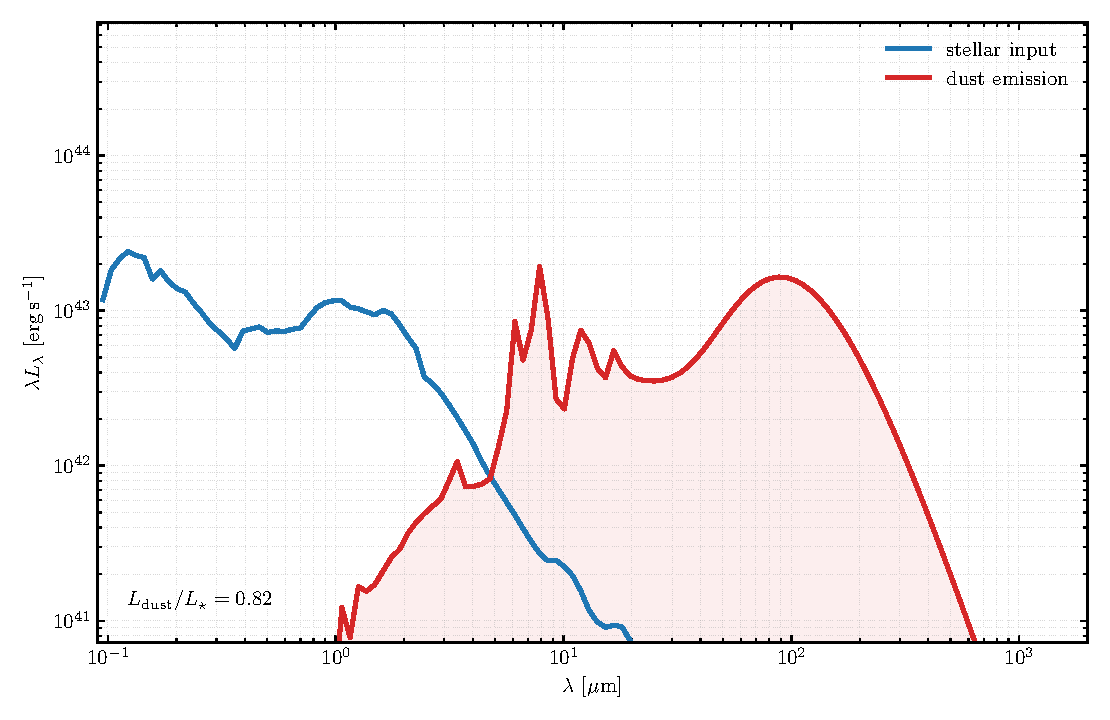
\includegraphics[width=\textwidth]{../examples/galaxy/galaxy_sed.pdf}
\end{minipage}\hfill
\begin{minipage}[b]{0.57\textwidth}
  \centering
  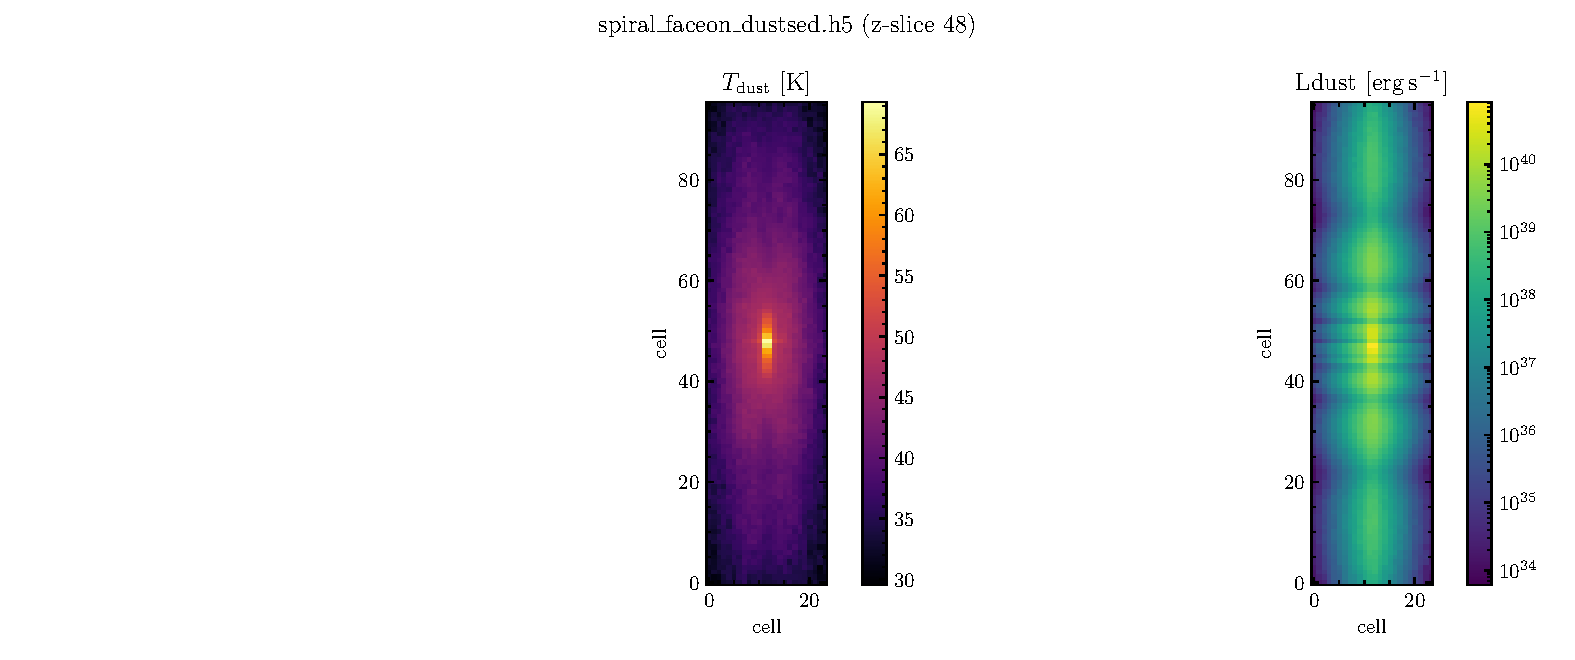
\includegraphics[width=\textwidth]{../examples/galaxy/spiral_faceon.pdf}
\end{minipage}
\caption{\emph{Left}: the UV-to-FIR SED of the \file{examples/galaxy} model
(exponential disk $+$ Sersic bulge): the attenuated starlight and the thermal
dust emission (PAH bands and a far-infrared peak), with $L_{\rm dust}/L_\star
\approx 0.8$.  \emph{Right}: the mid-plane dust-emission luminosity of the
\file{spiral\_faceon.in} model, showing the $m=2$ log-spiral arms imposed on the
dust density.}
\label{fig:galaxy}
\end{figure}

\begin{figure}[htb]
\centering
\begin{minipage}[t]{0.48\textwidth}
  \centering
  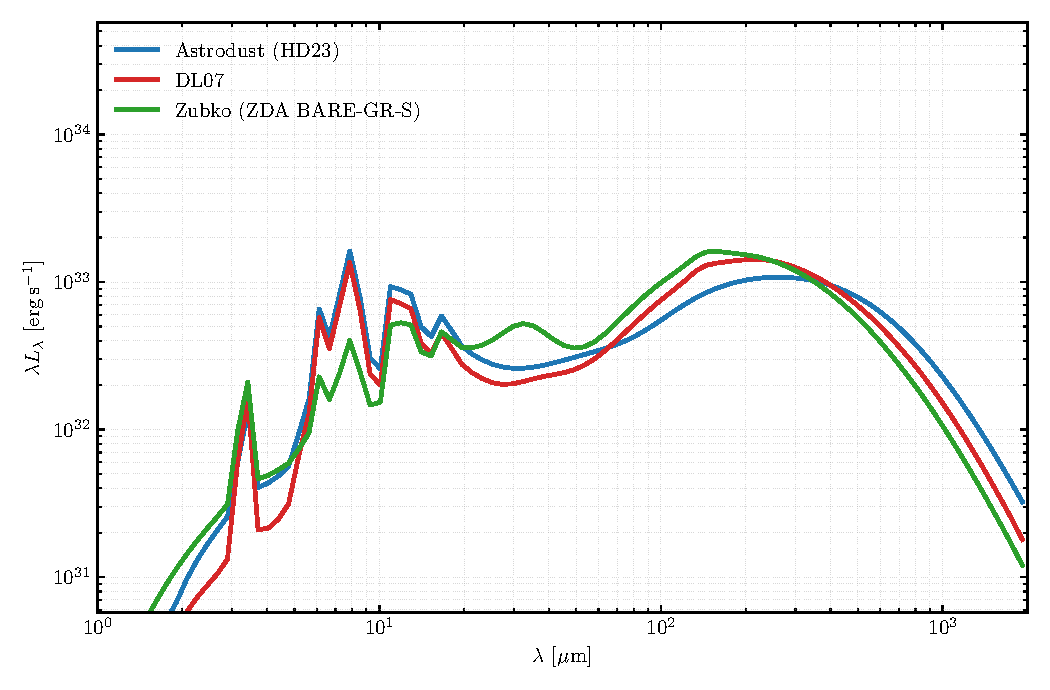
\includegraphics[width=\textwidth]{../examples/dustemis/dust_model_compare.pdf}
\end{minipage}\hfill
\begin{minipage}[t]{0.48\textwidth}
  \centering
  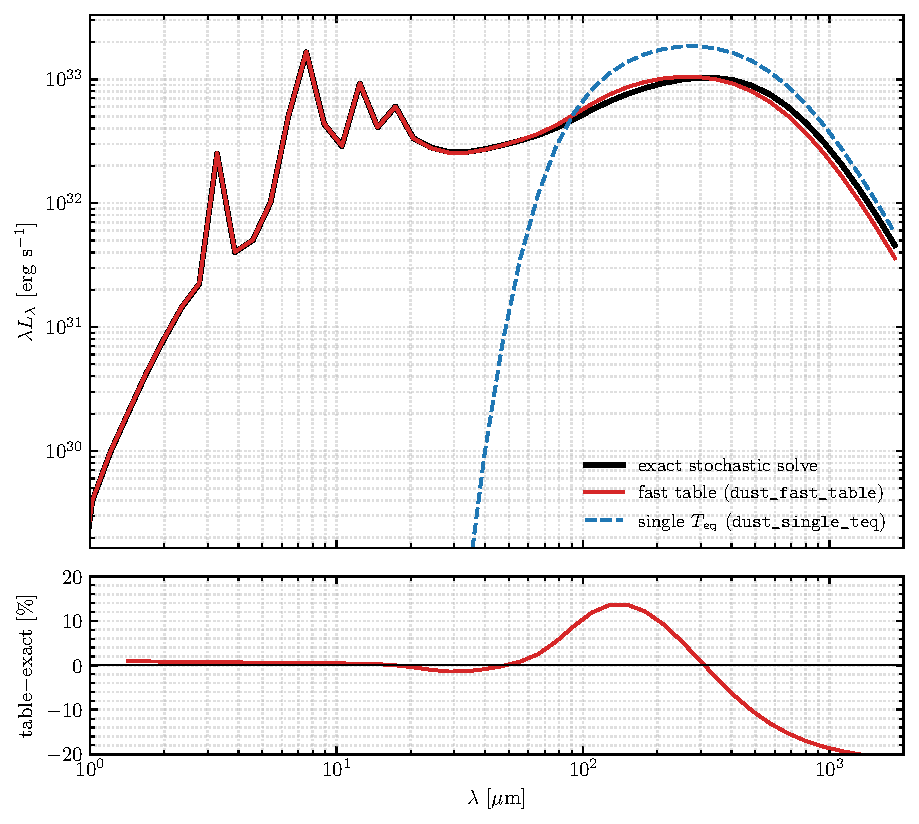
\includegraphics[width=\textwidth]{../examples/dustemis/table_accuracy.pdf}
\end{minipage}
\caption{\emph{Left}: the emission spectrum of a single cell heated by the same
radiation field, for the four \textsc{SEDust} grain models
(\code{astrodust}, \code{dl07}, \code{mrn}, \code{zubko}); the total power is identical (each
is normalized to the absorbed luminosity) while the PAH bands and the
far-infrared slope differ by model.  \emph{Right}: the \pp{dust\_fast\_table}
approximation against the exact stochastic solve --- the total luminosity is
identical, the PAH/mid-infrared region agrees to $\sim1\%$, and the largest
deviations sit on the far-infrared slope.}
\label{fig:dustmodels}
\end{figure}

\begin{figure}[htb]
\centering
\begin{minipage}[t]{0.48\textwidth}
  \centering
  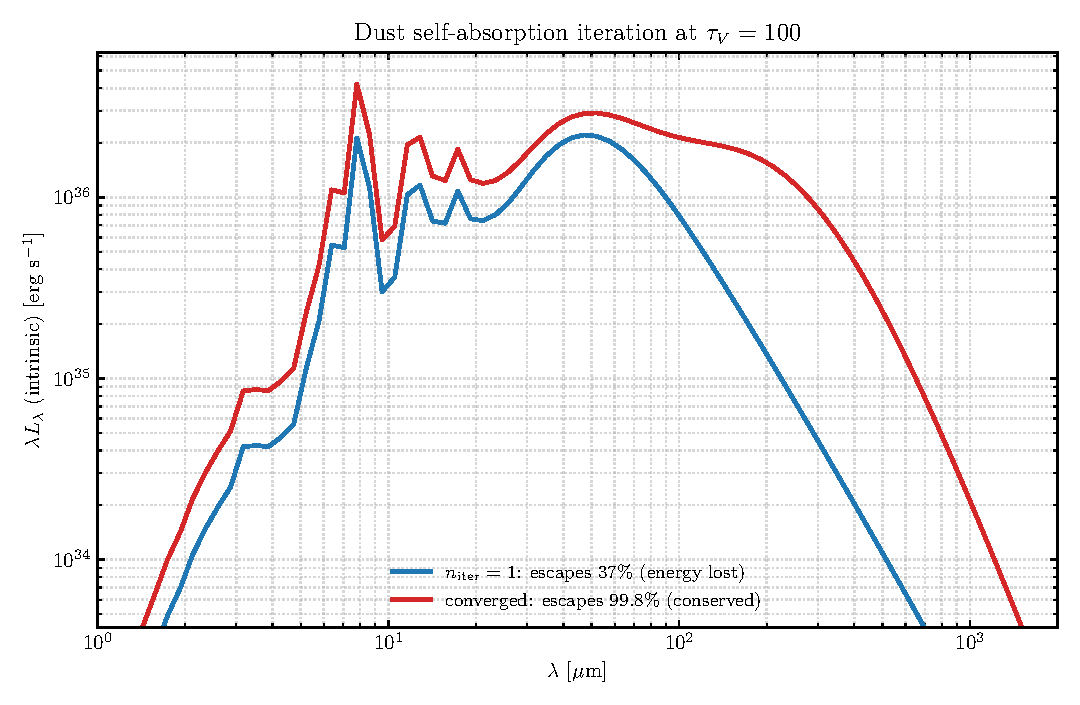
\includegraphics[width=\textwidth]{../examples/dustemis/iter_convergence.pdf}
\end{minipage}\hfill
\begin{minipage}[t]{0.48\textwidth}
  \centering
  \includegraphics[width=\textwidth]{../examples/milkyway/mw_cirrus.pdf}
\end{minipage}
\caption{\emph{Left}: convergence of the dust self-absorption iteration
(\pp{dust\_niter}) at $\tau_V=100$: the emitted luminosity converges
geometrically, and only the converged run conserves energy (a single pass loses
the reabsorbed dust emission).  \emph{Right}: the smoothed $8$--$500\,\mu$m
all-sky map from the interior-observer Milky-Way model
(\file{examples/milkyway}), a HEALPix Mollweide projection showing the
Galactic-plane concentration.}
\label{fig:iter}
\end{figure}

%=============================================================================
\section{Validation}
%=============================================================================
\begin{itemize}
\item \textbf{Regression.}  With the emission features off, the monochromatic
      scattering, the $(a,g)$/$\tau$ scans, and the clumpy-medium outputs are
      bit-identical to a stand-alone scattering run.
\item \textbf{Dust-emission engine (cross-code).}  Run through the
      \textsc{SEDust} library with the Zubko et al.~(2004) BARE-GR-S model, the
      emission spectra agree with the Camps et al.~(2015) seven-code
      stochastic-heating benchmark---which includes \textsc{SKIRT} and
      \textsc{DIRTY}---to a median relative difference of 2.5--4.4\% across
      $U=10^{-2}\ldots10^{4}$, inside the code-to-code envelope at every $U$,
      and the emission peak matches the code median to within one wavelength
      bin.
\item \textbf{Energy conservation.}  The intrinsic dust SED integrates to the
      absorbed luminosity to machine precision (the emission is normalized to
      the locally absorbed power).  The Lucy path-length estimator and the
      Bjorkman \& Wood immediate-reemission scheme agree on the absorbed
      luminosity to $<2\%$ over the sweep $\tau_V=0.1\ldots20$.
\item \textbf{AMR vs.\ Cartesian.}  Dust emission on a uniform level-5 octree
      sphere reproduces the reprocessed fraction ($0.863$ at $\tau_V=5$) and
      energy balance of the equivalent Cartesian sphere; Bjorkman \& Wood and
      MRW on the octree conserve energy identically.
\end{itemize}
\begin{figure}[htb]
\centering
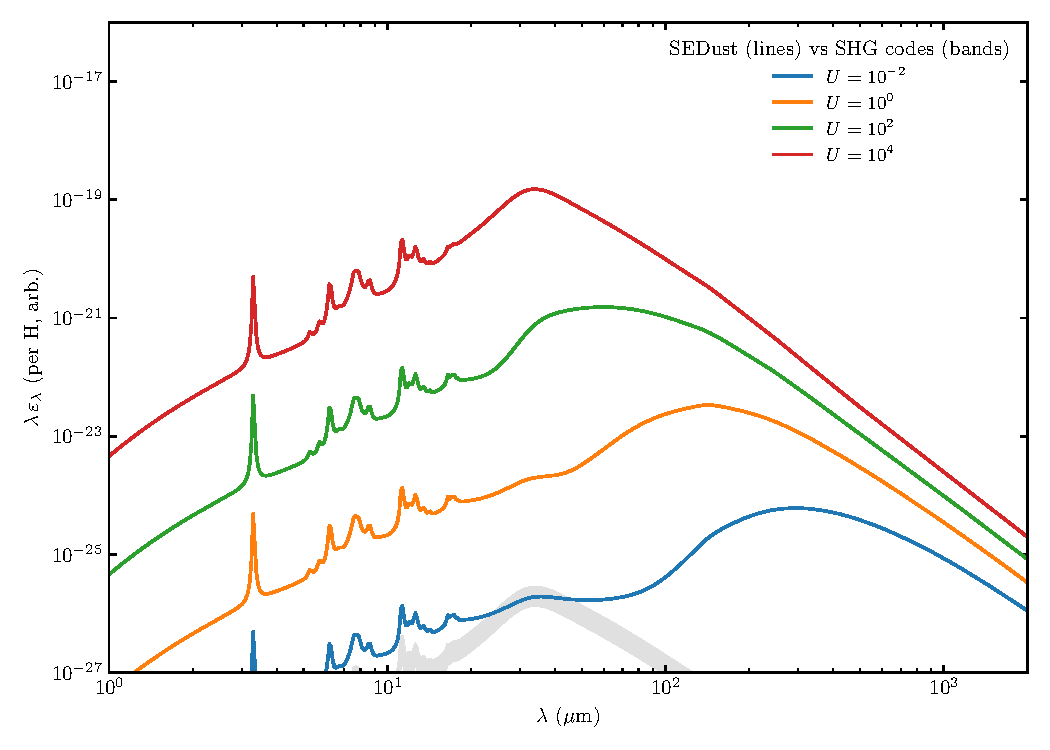
\includegraphics[width=0.7\textwidth]{../examples/benchmarks/shg_benchmark.pdf}
\caption{The \textsc{SEDust} single-cell emission spectrum (\code{zubko}
BARE-GR-S) against the Camps et al.~(2015) seven-code stochastic-heating
benchmark at several field strengths $U$; the shaded band is the code-to-code
spread, put on our own scale (the published spectra are in the benchmark's
units, so the comparison is of shape --- the level is set by the absorbed power
and is checked separately).  MoCafe tracks the benchmark median to a
2.5--4.4\% relative difference over $U=10^{-2}\ldots10^{4}$.}
\label{fig:shg}
\end{figure}

These checks are consolidated in \file{examples/benchmarks/validate.py}, which
re-runs the energy-conservation, two-method, and SHG cross-code tests and reports
PASS/FAIL.  External full-galaxy transport benchmarks (the TRUST slab, a direct
\textsc{SKIRT}/\textsc{DIRTY} image cross-check) need those codes or their
published reference solutions and are added as they become available; the
emission engine is already cross-checked against \textsc{SKIRT} and
\textsc{DIRTY} through the SHG benchmark above.

%=============================================================================
\section{Algorithm Notes}
%=============================================================================
\paragraph{Packet energy.}  Each packet carries a physical luminosity
$L_{\rm pk}$ [erg/s]: $L_\star/N_\star$ for stellar packets and
$L_{\rm dust}/N_{\rm dust}$ for dust-emission packets, so populations with
different packet energies combine correctly in the $J_\lambda$ tally.

\paragraph{Lucy iteration.}  The stellar $J_\lambda$ is tallied once and
reused; each iteration transports fresh dust-emission photons (sampled per cell
from the emission spectrum), adds their $J_\lambda$ to the stellar field, and
recomputes the emission.  The total emitted luminosity obeys
$L^{(k)}=L_{\rm abs}^\star + f\,L^{(k-1)}$ with $f$ the reabsorbed fraction, a
geometric series converging to $L_{\rm abs}^\star/(1-f)$.

\paragraph{Bjorkman \& Wood temperature.}  A cell's equilibrium temperature is
found by inverting the monotonic
$\kappa_B(T)=\int\!\kappa_{\rm abs}(\lambda)\,B_\lambda(T)\,d\lambda$ against
the running absorbed power per H nucleus.

%=============================================================================
\section*{References}
\addcontentsline{toc}{section}{References}
%=============================================================================
\begin{itemize}\small
\item Lucy, L.~B. 1999, A\&A, 344, 282 --- iterative mean-intensity /
      dust-emission estimator.
\item Bjorkman, J.~E. \& Wood, K. 2001, ApJ, 554, 615 --- immediate reemission
      with temperature correction.
\item Camps, P.\ et al. 2015, A\&A, 580, A87 --- stochastic-heating
      dust-emission benchmark.
\item Zubko, V., Dwek, E., \& Arendt, R.~G. 2004, ApJS, 152, 211 ---
      BARE-GR-S dust model.
\item Min, M.\ et al. 2009, A\&A, 497, 155; Robitaille, T.~P. 2010, A\&A, 520,
      A70 --- Modified Random Walk.
\item Seon, K.-I. 2010, PKAS, 25, 177 --- the $(a,g)$ single-run scan.
\item Jonsson, P. 2006, MNRAS, 372, 2 --- the polychromatic optical-depth scan.
\item G\'orski, K.~M.\ et al. 2005, ApJ, 622, 759 --- HEALPix pixelization
      (all-sky interior observer).
\item Amanatides, J. \& Woo, A. 1987, Eurographics~'87 --- fast voxel traversal.
\end{itemize}

\end{document}
